%%%%%%%%%%%%%%%%%%%%%%%%%%%%%%%%%%%%%%%%%%%%%%%%%%%%%%%%%%%%%%%%%%%%%%%%%%%%%
%
%  System        : 
%  Module        : 
%  Object Name   : $RCSfile$
%  Revision      : $Revision$
%  Date          : $Date$
%  Author        : $Author$
%  Created By    : Robert Heller
%  Created       : Mon Mar 11 19:32:20 2019
%  Last Modified : <190311.2029>
%
%  Description 
%
%  Notes
%
%  History
% 
%%%%%%%%%%%%%%%%%%%%%%%%%%%%%%%%%%%%%%%%%%%%%%%%%%%%%%%%%%%%%%%%%%%%%%%%%%%%%
%
%    Copyright (C) 2019  Robert Heller D/B/A Deepwoods Software
%			51 Locke Hill Road
%			Wendell, MA 01379-9728
%
%    This program is free software; you can redistribute it and/or modify
%    it under the terms of the GNU General Public License as published by
%    the Free Software Foundation; either version 2 of the License, or
%    (at your option) any later version.
%
%    This program is distributed in the hope that it will be useful,
%    but WITHOUT ANY WARRANTY; without even the implied warranty of
%    MERCHANTABILITY or FITNESS FOR A PARTICULAR PURPOSE.  See the
%    GNU General Public License for more details.
%
%    You should have received a copy of the GNU General Public License
%    along with this program; if not, write to the Free Software
%    Foundation, Inc., 675 Mass Ave, Cambridge, MA 02139, USA.
%
% 
%
%%%%%%%%%%%%%%%%%%%%%%%%%%%%%%%%%%%%%%%%%%%%%%%%%%%%%%%%%%%%%%%%%%%%%%%%%%%%%

\chapter{QuadSMCSenseHat: Quad Stall Motor Control and Sense HAT}

This is a circuit board for an add-on board for a Raspberry Pi B+ that will
control  four  stall-motor  turnout  motors for a model  railroad.  It also has
sense  logic to return the state of the  turnouts,  using one pole of the DPDT
contacts in the stall-motor (typical of Tortoise stall-motors).

The circuit board uses a 40pin header socket to connect to the 40pin header on
the  Raspberry Pi B+ and can use a  stack-through  header to allow  additional
boards to be stacked on top of it.

This uses a simplier (and probably cheaper) driver circuit, 
consisting of a pair of complementary MOS drivers to drive the stall-motor. 
This simplification uses so much less board space that it is possible to 
implement four driver and point sensors on a standard size Raspberry Pi 
``hat''.


\section{GPIO Pins Used and stacking restrictions.}

This board uses eight GPIO pins:

\begin{description}
\item[WiringPi 0, BCM 17] Motor Select 1: select the position of stall motor 
1. 
\item[WiringPi 1, BCM 18] Motor Select 2: select the position of stall motor 
2. 
\item[WiringPi 2, BCM 27] Point Sense 1: return the state of the points for 
stall motor 1. 
\item[WiringPi 3, BCM 22] Point Sense 2: return the state of the points for 
stall motor 2. 
\item[WiringPi 4, BCM 23] Motor Select 3: select the position of stall motor 
3. 
\item[WiringPi 5, BCM 24] Motor Select 4: select the position of stall motor 
4. 
\item[WiringPi 6, BCM 25] Point Sense 3: return the state of the points for 
stall motor 3. 
\item[WiringPi 7, BCM 4] Point Sense 4: return the state of the points for 
stall motor 4. 
\end{description}

Only one board of this type can be used on a given Raspberry Pi because of the 
hard-wired GPIO pin usage.

\section{Circuit Description}

\begin{figure}[hbpt]\begin{centering}%
\includegraphics[width=5in]{QuadSMCSenseHat.pdf}
\caption{Circuit Diagram of the QuadSMCSenseHat}
\end{centering}\end{figure}
This circuit contains two sections.  There is an output section that contains 
a dual complementary MOSFET driver (one inverting, one non-inverting) for each 
motor.  The other section contains pairs of NAND gates wired as RS Flip Flops 
that debounce and buffer/store point state.  Each GPIO output pin drives its 
pair of MOSFET drivers, and since one of the pair in inverting and the 
non-inverting only one of the drivers is activated when the GPIO output pin is 
high and the other is activated when the GPIO output pin is low.  

The other section is four flip-flop debounce circuits, one for each of four
SPDT switch contacts that report the position of the turnout points. The
output of these flip-flops goes to the four GPIO input pins.

\section{Parts List}

\begin{table}[htdp]
\begin{centering}\begin{tabular}{|l|l|p{1in}|l|}
\hline
Value&Qty&Refs&Mouser Part Number \\
\hline
.1 uf&2&C1 C2&581-SR201C104KARTR1\\
\hline
10 uf 35V&1&C3&667-ECA-1HM100I\\
\hline
RPi\_GPIO&1&J0&855-M20-6102045\\
\hline
10K Ohms&1&RR1&652-4609X-1LF-10K\\
\hline
Motor 1;Motor 2;Motor 3;Motor 4&4&T1 T2 T3 T4&651-1725685\\
\hline
+ 12V -&1&T5&651-1725656\\
\hline
TC4428&4&U1 U2 U3 U4&579-TC4428VPA\\
\hline
74HCT00&2&U5 U6&595-SN74AHC00N\\
\hline
\end{tabular}
\caption{Parts list for QuadSMCSenseHat boards.}
\end{centering}\end{table}

The only parts that might be substituted are J0 (the RPi GPIO Header), and T1
through T4 (the Motor terminals) and T5 (the 12 to 16 Volts terminals). The
parts listed are for the stacking headers for the RPi GPIO Header, and screw
terminals for the Motor terminals and the motor power terminals. Feel free to
select a non-stacking header for the RPi GPIO Header and to select either pin
arrays or spring terminals for the T1 through T5 (any 2.54 pitch inline 
terminals or connectors)\footnote{Mouser Project link: 
\url{http://www.mouser.com/ProjectManager/ProjectDetail.aspx?AccessID=330542c522}.}.

\section{Circuit Board Layout}

\begin{figure}[hbpt]\begin{centering}%
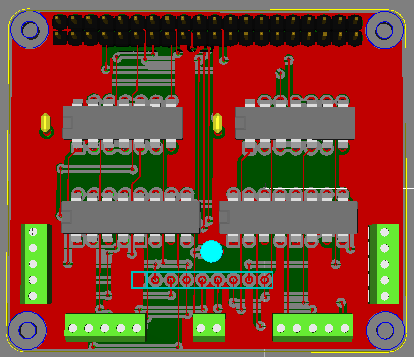
\includegraphics[width=5in]{QuadSMCSenseHat3DTop.png}
\caption{3D rendering of the QuadSMCSenseHat board}
\end{centering}\end{figure}
\begin{figure}[hbpt]\begin{centering}%
\includegraphics[width=5in]{QuadSMCSenseHat.png}
\caption{Fabrication image of the QuadSMCSenseHat board}
\end{centering}\end{figure}
Board assembly is straight forward.  You need to be careful orienting the ICs, 
and the electrolytic capacitor.  And don't forget to orient the screw 
terminals with the wire entries facing out from the board!

\section{Downloadables and Software Support}

Full design information is available on GitHub here:                           
 
\url{https://github.com/RobertPHeller/RPi-RRCircuits/tree/master/QuadSMCSenseHat}.

An OpenMRN program is available on GitHub here:

\url{https://github.com/RobertPHeller/RPi-RRCircuits/tree/master/QuadSMCSenseOpenMRN}.

Also, bare boards can be ordered from Pcbway here:

\url{https://www.pcbway.com/project/shareproject/Quad_Stall_Motor_Controller_w__point_Sense__hat_.html}.




